\section{MÉTODO}

Segundo \citeonline{php5ConceitosProgramacaoEIntegracaoComBancoDeDados}, um
método pode ser definido como sendo as operações que manipulam os dados de uma 
classe, ou seja, definem o que as classes podem e sabem fazer, como por exemplo 
acelerar um carro modificando o valor de sua propriedade chamada 
\textit{velocidade} para um valor crescente em um determinado espaço de tempo.

Os métodos também podem ser chamados de funções membro \cite{c++ComoProgramar}.

Se comparado a programação estruturada um método pode ser considerado como sendo
uma função que está associada a uma classe \cite{programmingPhp}.

\begin{figure}[h!tb]
	\caption{Criação de um Método utilizando a linguagem PHP}
	\label{fig:metodo}
	
	\centering
	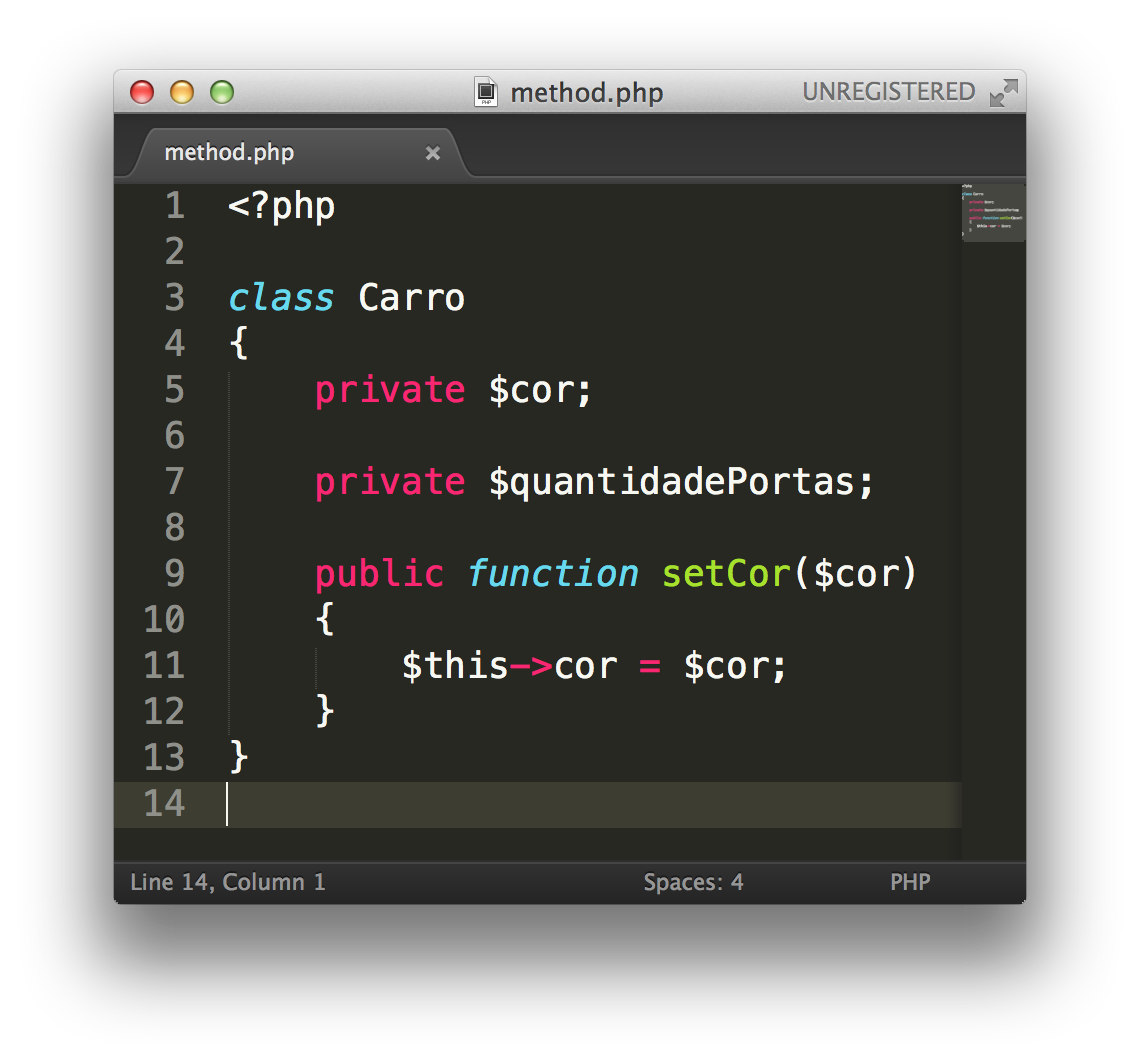
\includegraphics[width=0.75\textwidth]{images/method.png}
	
	\centering
	\footnotesize Fonte: \fonteOAutor
\end{figure}

\FloatBarrier 	% Este comando impede que as imagens 
				% flutuem a partir deste ponto no seu documento

Na sequência, você irá conferir uma explicação referente ao código que foi
apresentado na figura \ref{fig:metodo}:

\begin{enumerate}[a)]
    \item \textbf{linha 1:} temos o início da execução de um bloco de código PHP;
    \item \textbf{linha 3:} definimos uma classe chamada \textit{Carro};
    \item \textbf{linha 4:} definimos onde inicia o bloco de uma classe;
    \item \textbf{linha 5 e 7:} definimos duas propriedades para a classe
    \textit{Carro}, são elas: \textit{\$cor} e \textit{\$quantidadePortas};
    \item \textbf{linha 9:} é solicitado para que o interpretador crie um método
    cuja visibilidade seja pública (falaremos sobre isso ainda neste capítulo) 
    e definimos que este método será identificado pelo nome \textit{setCor}.
    Além disso, dizemos que este método deve receber um parâmetro (um valor 
    que  irá configurar a propriedade de uma classe);
    \item \textbf{linha 10:} definimos onde inicia o bloco cujo escopo
    corresponda ao método \textit{setCor};
    \item \textbf{linha 11:} usamos uma variável especial chamada
    \textit{\$this}, esta variável permite acessar qualquer propriedade ou
    método dentro da própria classe ou superclasses; depois, utilizamos o 
    operador de acesso a um objeto (representado pelo símbolo \textbf{->}); em
    seguida, informamos que vamos manipular o valor da propriedade \textit{cor}
    e que ela receberá o valor informado como parâmetro para o método \textit{setCor};
    \item \textbf{linha 12:} definimos onde termina o bloco que corresponde ao
    método \textit{setCor};
    \item \textbf{linha 13:} definimos onde termina o bloco de uma classe.
\end{enumerate}
				
Isto permite que de fora da classe carro outro objeto configure a cor de um
veículo passando uma mensagem ao objeto carro com a cor solicitada. Podemos ver 
um exemplo desta situação na imagem abaixo:


\begin{figure}[h!tb]
	\caption{Chamada de um Método utilizando a linguagem PHP}
	\label{fig:chamadaMetodo}
	
	\centering
	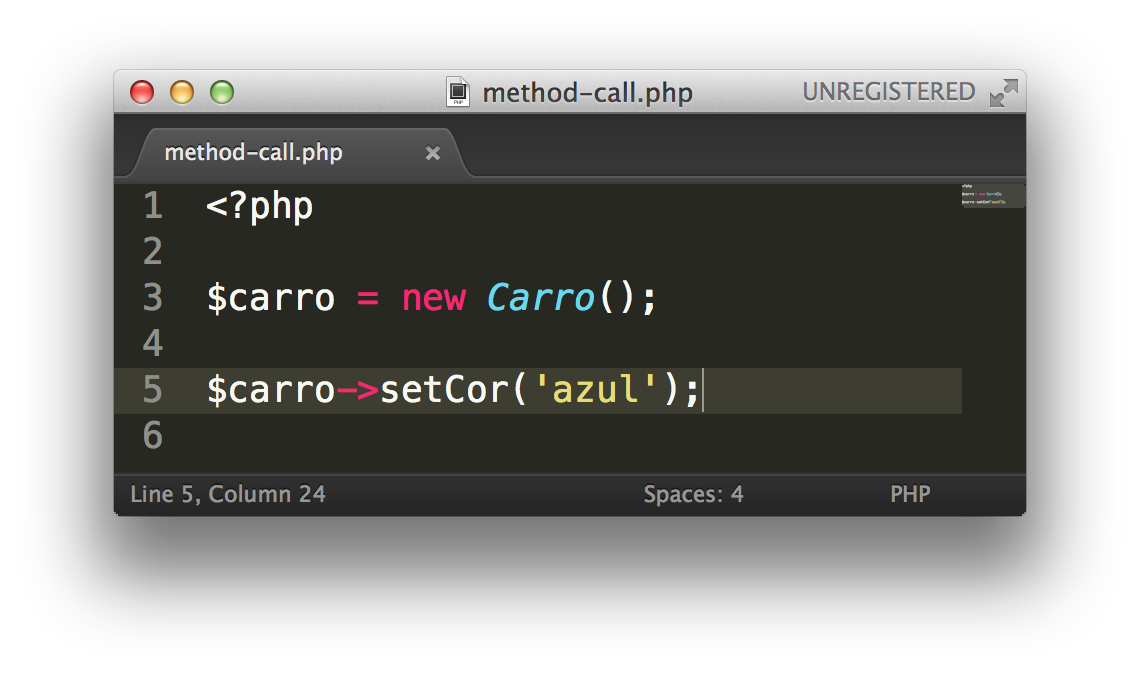
\includegraphics[width=0.75\textwidth]{images/method-call.png}
	
	\centering
	\footnotesize Fonte: \fonteOAutor
\end{figure}

\FloatBarrier 	% Este comando impede que as imagens 
				% flutuem a partir deste ponto no seu documento

Abaixo, você irá conferir uma explicação referente ao código que foi
apresentado na figura \ref{fig:chamadaMetodo}:

\begin{enumerate}[a)]
    \item \textbf{linha 1:} temos o início da execução de um bloco de código
    PHP;
    \item \textbf{linha 2:} temos a criação de um objeto do tipo \textit{Carro};
    \item \textbf{linha 5:} temos a chamada de um método chamado
    \textit{setCor}, sendo que, informamos um parâmetro para ele, que na 
    linguagem PHP representa uma string (cadeira de caracteres). Logo, estamos 
    configurando o valor da propriedade da classe \textit{Carro} \textit{cor}
    para receber o valor \textit{azul}.
\end{enumerate}